

\documentclass[DIV=calc, paper=a4, fontsize=10.5pt]{scrartcl}
\usepackage{makeidx}
\usepackage{graphicx}
\usepackage{flushend}
\usepackage{amssymb}


\usepackage{lmodern}
\usepackage[left=1.5cm,right=1.5cm,top=2.5cm,bottom=2cm]{geometry}
\usepackage{float}		
\bibliographystyle{plain} 
\pagestyle{plain} 
\pagenumbering{arabic}
\usepackage{fancyhdr} 	
\usepackage[T1]{fontenc}
\usepackage[utf8]{inputenc}
\usepackage[spanish]{babel}
\usepackage[spanish,es-tabla]{babel}
\usepackage{hyperref}
\usepackage{graphicx}
\usepackage{siunitx}
\usepackage{lipsum}
\usepackage[protrusion=true,expansion=true]{microtype}
\usepackage{amsmath,amsfonts,amsthm}
\usepackage[svgnames]{xcolor}
\usepackage[svgnames]{xcolor}
\usepackage{booktabs}
\usepackage{fix-cm}
\usepackage{multicol}
\usepackage{url}
\usepackage{cancel}
\usepackage{subfig}
\bibliographystyle{unsrt}

\newenvironment{Figura}
  {\par\medskip\noindent\minipage{\linewidth}}
  {\endminipage\par\medskip}

\usepackage{sectsty}
\allsectionsfont{\usefont{OT1}{phv}{b}{n}}
\usepackage{fancyhdr}
\spanishdecimal{.}
\pagestyle{fancy}
\usepackage{lastpage}
\lhead{}
\chead{}
\rhead{}
\lfoot{}
\cfoot{}
\rfoot{\footnotesize Page \thepage\ of \pageref{LastPage}}
\renewcommand{\headrulewidth}{0.0pt}
\renewcommand{\footrulewidth}{0.4pt}
\usepackage{lettrine}
\newcommand{\initial}[1]{\lettrine[lines=3,lhang=0.3,nindent=0em]{
\color{DarkGoldenrod}{\textsf{#1}}}{}}
\usepackage{titling}
\newcommand{\HorRule}{\color{DarkGoldenrod} \rule{\linewidth}{1pt}}
\pretitle{\vspace{-120pt} \begin{flushleft} \HorRule \fontsize{22}{35} \usefont{OT1}{phv}{b}{n} \color{DarkRed} \selectfont}
\title{Práctica 11. \\ %Aquí va el nombre de la práctica 
Interferometro de Michelson} %Numero de la práctica 
\posttitle{\par
\end{flushleft}
\vskip 0.5em}
\preauthor{\begin{flushleft}\large \lineskip 0.5em \usefont{OT1}{phv}{b}{sl} \color{DarkRed}}
\author{Angel Yair García Pérez \\
Misael Iván Macías Márquez\\
Teodora Irene Ortíz Cruz\\
\small{teodora625@ciencias.unam.mx}\\}
\postauthor{\footnotesize \usefont{OT1}{phv}{m}{sl} \color{Black}
\vspace*{0.1cm} 
Facultad de Ciencias, UNAM
\par\end{flushleft}\HorRule}
\date{9 de Junio de 2022\\Semestre 2022-2}
\begin{document}
\maketitle
\definecolor{carmine}{rgb}{0.59, 0.0, 0.09}
\begin{abstract}

  \textcolor{carmine}{Resumen:} Usando un interferómetro, se contó el número de franjas vistas a una distancia recorrida por el tornillo micrométrico y con esos datos se obtuvo la constante de proporcionalidad del interferómetro $k = 4.74 \pm 1.93\times 10^{-13}$ la cual entra en el rango de valores $(4,6)$ con una  incertidumbre relativa $\Delta_{\%} = 4\times 10^{-12}\%$ y la longitud de onda de un láser amarillo $\lambda_{\text{amarillo}} = (580 \pm 50) \text{ nm}$ con una discrepancia de $0.28\hspace{0.1cm}<\hspace{0.1cm}2$ y una incertidumbre  $\Delta_{\%}=8.6\%$. Luego se utilizó un detector conectado al osciloscopio y se contaron lo picos que se veían en la pantalla del osciloscopio, en el momento en que se movió el tornillo micrométrico. Con este método se obtuvo que la constante de proporcionalidad era de $k= 4.49 \pm 2.91 \times 10^{-14}$ la cual entra en el rango de valores $(4,6)$  con incertidumbre  $\Delta_{\%} = 6 \times 10^{-13}\%$ y que la longitud de de onda del láser amarillo era de $\lambda_{\text{amarillo}} = (595 \pm 10) \text{ nm}$ con una discrepancia de $(0.1\hspace{0.1cm}<\hspace{0.1cm}2)$ y una $\Delta_{\%}=1.68\%$. Con base en lo anterior, se considera que los resultados del experimento fueron satisfactorios.
\end{abstract}
\section*{\textcolor{carmine}{Introducción.}}
El objetivo de este trabajo es caracterizar el factor de proporcionalidad de un interferómetro de Michelson y practicar el uso para calcular longitudes de onda monocromáticas \cite{Manual}. La importancia de está practica radica en familiarizarse con el interferómetro uno de los instrumentos experimentales más importantes y también aprender a utilizar un osciloscopio, destacando que se debe saber utilizar la tecnología de manera adecuada \cite{Manual}. Se espera que se cumpla el modelo teórico propuesto en la literatura \cite{book} para obtener un factor de proporcionalidad  del interferómetro entre el rango (4,6) y con base a los valores de la hoja de datos del láser amarillo, utilizando las constante de proporcionalidad obtenida antes, se espera encontrar que el valor de la longitud de onda para el láser amarillo sea de $594.1\text{ nm}$. 
\subsection*{\textcolor{carmine}{Interferómetro}}
El interferómetro es un dispositivo experimental diseñado por Albert Michelson mientras estaba en busca del éter. Consiste en un arreglo de espejos colocados en L, como se muestra en la Figura 1(a), y en el centro se coloca un divisor de haz  y una placa de vidrio\cite{book}. Si a dichos dispositivo experimental se le incide un haz de luz se puede llevar acabo un diagrama de rayos como el de la Figura 1(b) y usando la geometría del diagrama de rayos y la ecuación para espejos planos se obtiene una ecuación de camino óptico camino óptico es\cite{Manual}.
Haciendo uso de los conceptos de interferencia se obtienen condiciones de interferencia constructiva $\Delta_{co}=m\lambda$ y destructiva $\Delta_{co}+\Delta_{r}=\left(\frac{1}{2}+m\right)\lambda$. Debido a la simetría circular al rededor del eje óptico se produce un sistema de anillos de interferencia como el que se muestra en la Figura 1(a). Finalmente so obtiene que la interferencia destructiva esta dada por\cite{book}
\begin{equation*}
    2\Delta_{d}\cos{\theta}=m\lambda
\end{equation*}
considerando $\theta=0$ para estudiar el patrón de los anillos se tiene que la ecuación anterior es 
\begin{equation*}
    2\Delta_{d}=m\lambda
\end{equation*}
Si se considera m como el número de anillos se obtiene que la longitud de onda es 
\begin{equation*}
    \lambda=\frac{2\Delta}{N}
\end{equation*}
En la practica se debe de tomar en cuenta que los interferómetros tienen un factor de proporcionalidad $k$ del reductor y que la distancia medida será la que se desplazó el micrómetro $d'$. La ecuación del factor de proporcionalidad del interferómetro es\cite{Manual}
\begin{equation}
    k=\frac{2d'}{N\lambda}
\end{equation}
\begin{figure}
 \centering
  \subfloat[Esquema de un interferómetro de Michelson\cite{book}]{
   \label{f:gato}
    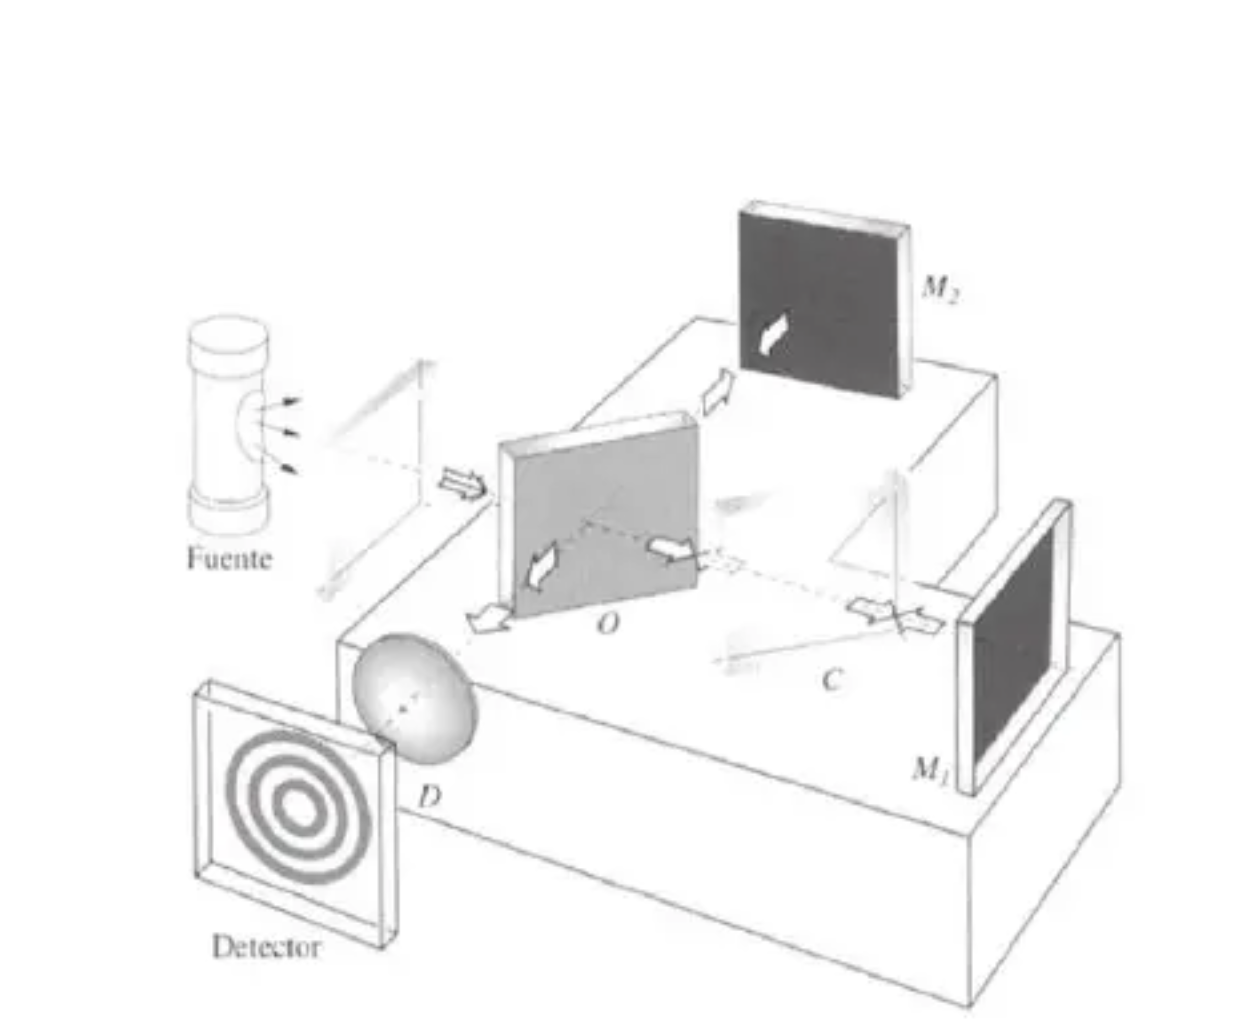
\includegraphics[width=0.3\textwidth]{Captura de Pantalla 2022-06-02 a la(s) 15.18.53.png}}
  \subfloat[Diagrama de Rayos de un interferómetro de Michelson\cite{book}]{
   \label{f:tigre}
    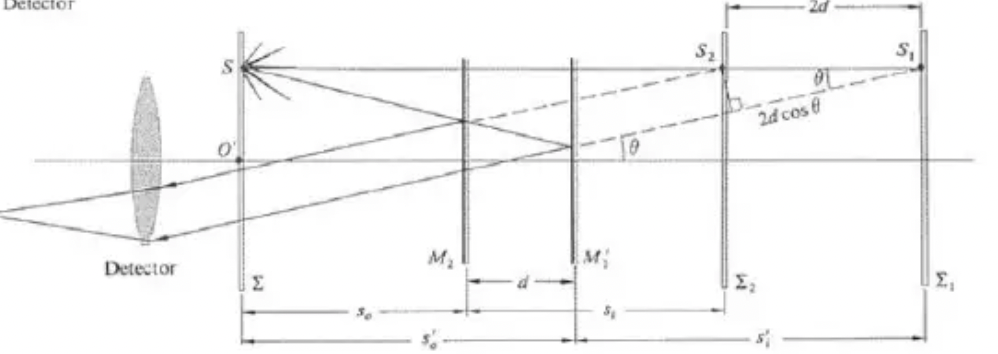
\includegraphics[width=0.4\textwidth]{Captura de Pantalla 2022-06-02 a la(s) 15.25.42.png}}
    \caption{Esquemas para poder visualizar mejor la teoría expuesta, en el 1(a) Se puede observar el interferómetro descrito junto con el patrón de anillos que produce. En la figura 1(b) se observa el diagrama de rayos que sirve para poder construir las ecuaciones del interferómetro.}
 \label{f:animales}
\end{figure}
\section*{\textcolor{carmine}{Desarrollo Experimental.}}
Sobre la mesa del laboratorio se colocó un interferómetro y frente a el se puso un láser de tubo rojo en una base, este se encendió y se nivelo de tal manera en que el haz atravesara por el centro de los espejos, esto hizo que en la pared del laboratorio se vieran puntitos de luz lo que indicaba que el haz había sido dividido por el divisor del interferómetro. Se giraron los tornillos posteriores hasta que se vieran empalmados los dos haces de luz. Después entre el interferómetro y el láser se colocó un objetivo de microscopio montado en un porta lentes, como se muestra en la Figura 2, provocando que se vieran anillos luego se centraron los anillos y se colocó el tornillo micrométrico en el cero.\\
Con lo anterior ya hecho, cada uno de los integrantes del equipo contó alrededor de 30 a 40 franjas mientras se movía el tornillo micrométrico cuidadosamente. Al finalizar el conteo se tomaba la medida de cuanto se había desplazado el tornillo considerando una incertidumbre $\sigma_{ap}=\hspace{0.1cm}\pm \hspace{0.1} 5 \hspace{0.1cm}\mu m$.\\
Luego se cambió el láser rojo por un láser amarillo y se repitió el mismo procedimiento considerando que con la parte anterior se obtuvo el factor de proporcionalidad.\\
\begin{figure}[H]
    \centering
    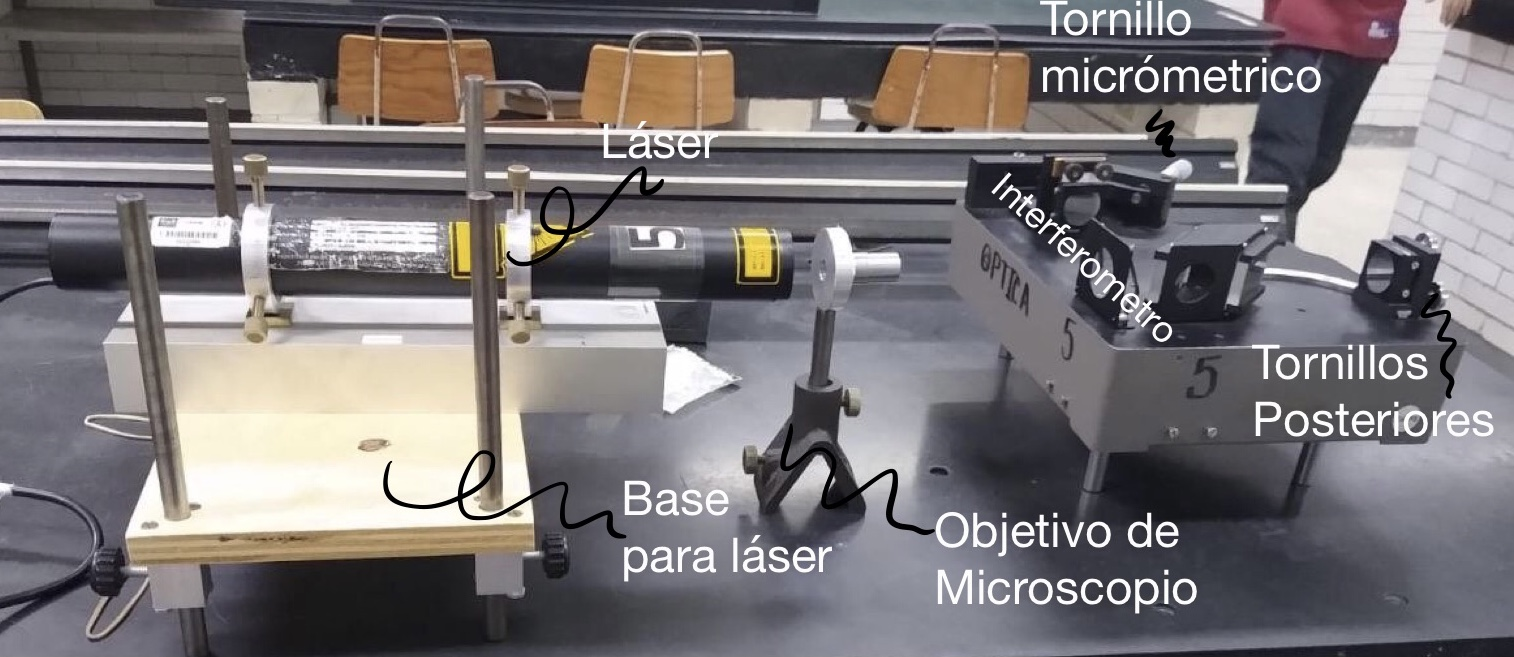
\includegraphics[width=9cm]{Imagenes/6369C4D1-A2A9-423F-B344-6F347043CD72.jpeg}
    \caption{Arreglo experimental para obtener la constante de proporcionalidad y la longitud de onda de un láser amarillo a partir de contar el número de franjas.}
    \label{fig:my_label}
\end{figure}
\newpage
\textbf{\textcolor{carmine}{Uso del osciloscopio.}}\\

Sobre la mesa del laboratorio se colocó un osciloscopio y el mismo arreglo experimental ya alineado de la parte anterior, sin el objetivo de microscopio. Para este caso se conectó un detector al osciloscopio y se colocó frente al haz que se proyectaba en la pared como se muestra en la Figura 3. Con el osciloscopio encendido se esperó a que la señal se estabilizara y se fue modificando la escala conforme esta crecía o decrecía. Luego se movió el tornillo micrométrico del interferómetro hasta estar en cero. Con el arreglo experimental preparado uno de los integrantes del equipo movió el tornillo cuidadosamente y con el mejor pulso posible, mientras que el otro pulsaba el botón de "Stop" para obtener el patrón de interferencia arrojado por el osciloscopio. Luego se hizo zoom y se contó el número de picos que había en la señal, esto se repitió por cada miembro del equipo. Para medir la distancia que se movió el tornillo micrométrico se considero una incertidumbre de apreciación $\sigma_{ap}=\hspace{0.1cm}\pm \hspace{0.1} 5 \hspace{0.1cm}\mu m$. 
\begin{figure}[H]
    \centering
    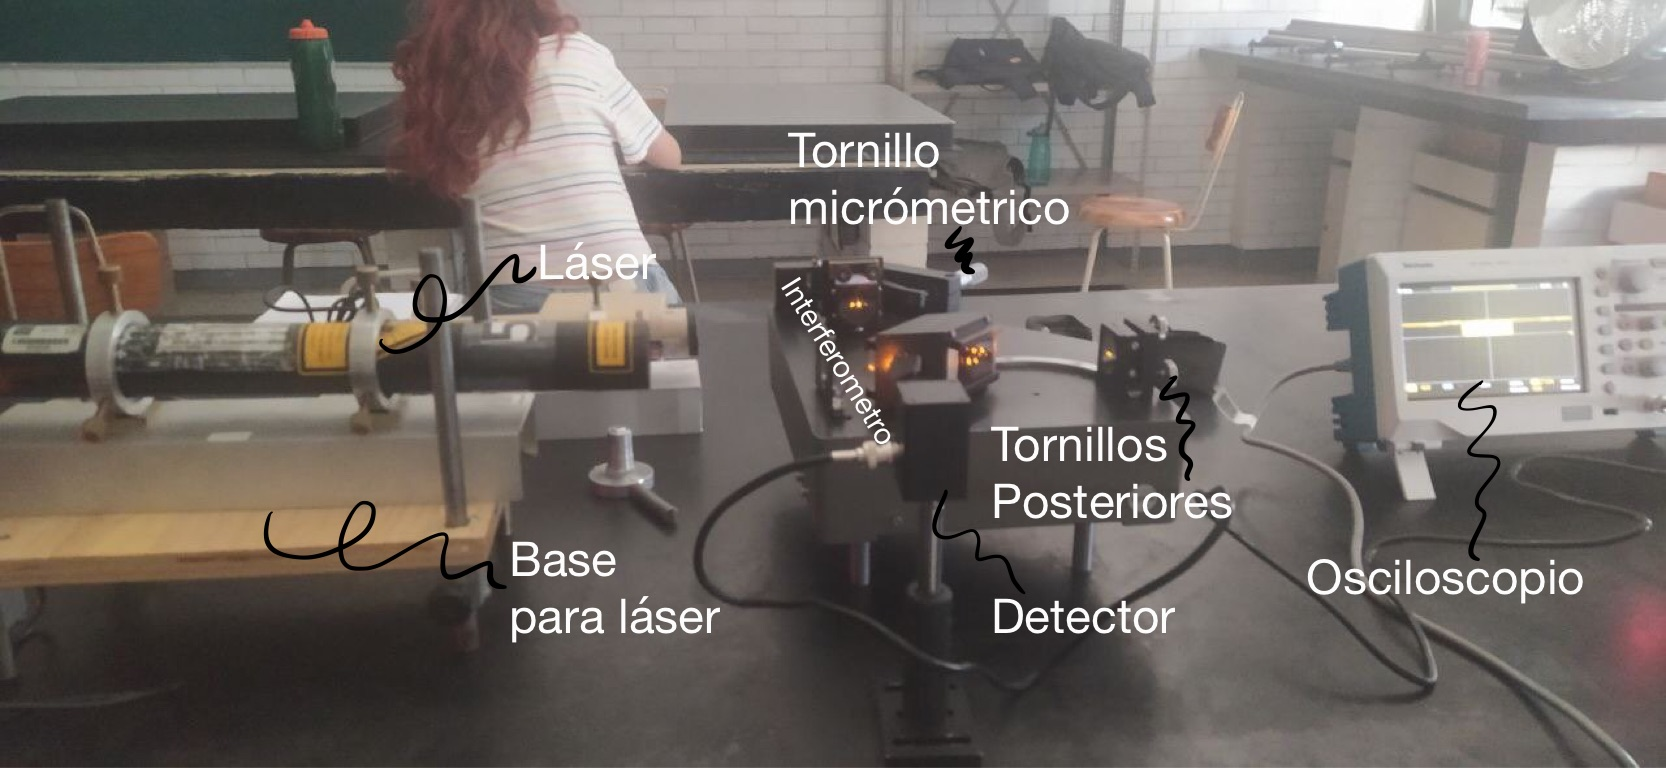
\includegraphics[width=9cm]{Imagenes/BC685A71-84C3-4F1D-8218-2F34C8B42734.jpeg}
      \caption{Arreglo experimental para obtener la constante de proporcionalidad y la longitud de onda de un láser amarillo a partir de contar el número de picos obtenidos en la señal del osciloscopio.}
    \label{fig:my_label}
\end{figure}


\section*{\textcolor{carmine}{Resultados y Análisis.}}

Propagando la incertidumbre de la ecuación (2) se tiene,

\begin{equation*}
    \Delta k = \left|\frac{\partial k}{\partial d'}\right| \Delta d'= \frac{2\Delta d'}{N\lambda}
\end{equation*}

Las constantes de proporcionalidad obtenidas son las siguientes:

\begin{figure}[H]
    \centering
    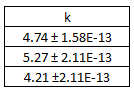
\includegraphics{tablas/tabla 1.PNG}
    \caption{Tabla de constantes de proporcionalidad.}
    \label{fig:my_label}
\end{figure}

El promedio de las constantes de proporcionalidad  da un valor de:

\begin{equation*}
    k = (4.74 \pm 1.93\times 10^{-13})
\end{equation*}


Despejando $\lambda$ de la ecuación (2) y propagando su incertidumbre se tiene,

\begin{equation*}
    \Delta \lambda = \sqrt{ \left(\frac{\partial \lambda}{\partial d'} \Delta d'\right)^{2} + \left(\frac{\partial \lambda}{\partial k} \Delta k\right)^{2}} = \frac{2d'}{Nk} \sqrt{\left(\frac{\Delta  d'}{d'}\right)^{2} + \left(\frac{\Delta k}{k}\right)^{2}}
\end{equation*}

Las longitudes de onda obtenidas son las siguientes:

\begin{figure}[H]
    \centering
    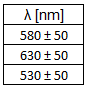
\includegraphics{tablas/tabla 2.PNG}
    \caption{Tabla de longitudes de onda para el láser naranja.}
    \label{fig:my_label}
\end{figure}

El promedio de las longitudes de onda da un valor para el láser naranja de:

\begin{equation*}
    \lambda_{\text{naranja}} = (580 \pm 50) \text{ nm}
\end{equation*}

Con el osciloscopio se obtuvieron las siguientes constantes de proporcionalidad:

\begin{figure}[H]
    \centering
    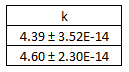
\includegraphics{tablas/tabla 3.PNG}
    \caption{Tabla de constantes de proporcionalidad obtenidas con el osciloscopio.}
    \label{fig:my_label}
\end{figure}

El promedio de las constantes de proporcionalidad  da un valor de:

\begin{equation*}
    k = (4.49 \pm 2.91\times 10^{-14})
\end{equation*}

Las longitudes de onda obtenidas son:

\begin{figure}[H]
    \centering
    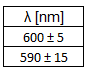
\includegraphics{tablas/tabla 4.PNG}
    \caption{Longitudes de onda obtenidas con el osciloscopio para el láser naranja.}
    \label{fig:my_label}
\end{figure}

El promedio de las longitudes de onda da un valor para el láser naranja de:

\begin{equation*}
    \lambda_{\text{naranja}} = (595 \pm 10) \text{ nm}
\end{equation*}



\section*{\textcolor{carmine}{Discusión y Conclusión.}}

Se obtuvo que la constante de proporcionalidad del interferómetro es: 
$$k = 4.74 \pm 1.93\times 10^{-13}$$
La constante de proporcionalidad entra en el rango de valores $(4,6)$ esperado, este rango se presentó en la introducción.
\\
Se encontró que la longitud de onda del láser amarillo es:
$$\lambda_{\text{naranja}} = (580 \pm 50) \text{ nm}$$
Con ayuda del osciloscopio se obtuvo que la constante de proporcionalidad es:
$$k= 4.49 \pm 2.91 \times 10^{-14}$$ 
La cual entra en el rango de valores $(4,6)$
\\
Se encontró que la longitud de onda del láser amarillo es:
$$\lambda_{\text{naranja}} = (595 \pm 10) \text{ nm}$$
Los valores de la longitud de onda concuerdan con el valor esperado presentado en la introduccion $594.1 nm$.
\\
Los valores obtenidos con ayuda del osciloscopio son mas precisos, ya que se disminuyen los errores al contar el número de franjas de interferencia detectadas por este.
\nocite{*}

\bibliography{biblio}

\end{document}